\documentclass{beamer}
%\documentclass[xcolor=pst,dvips,epic,eepic]{beamer}

\usepackage[utf8]{inputenc}
\usetheme{Singapore}
\usepackage{xcolor}
\setbeamertemplate{footline}[frame number]

\usepackage{mathlist}

\usepackage{amsmath,amssymb, amsthm}
\usepackage{amscd}

%\newtheorem{theo}{Théorème}

\usepackage{pstricks, pst-node}

\usepackage{times}

\usepackage{ulem}

\usepackage{listings}
%\topmargin=-0.6in
\lstloadlanguages{C++}
\lstset{language=C++}
%%}

\setbeamercovered{dynamic}

\def\bxi{\boldsymbol\xi}
\def\bomega{\boldsymbol\omega}
\def\bC{\boldsymbol{C}}
\def\bu{\boldsymbol{u}}
\def\bU{\boldsymbol{U}}
\def\bu{\boldsymbol{u}}
\def\by{\boldsymbol{y}}
\def\vol{\mbox{vol}}

\title[Random Numbers Generation]{A short tutorial of random numbers generation}

\author[Fabian Bastin]{Fabian Bastin \\ \url{fabian.bastin@umontreal.ca} \\ Université de Montréal -- CIRRELT -- IVADO -- Fin-ML}
\date{}

\begin{document}
	
	\frame{\titlepage}
	
	%\begin{frame}
	%\frametitle{Outline}
	%
	%\end{frame}
	
	\begin{frame}
		\frametitle{U[0,1]-distributed random numbers}
		
		\begin{itemize}
			\item
			A good uniform random generator on the interval $[0,1]$ is a major
			component of any good random generator library.
			\item
			Draws from other distributions are usually obtained by adequately transform an
			uniformly distributed sample.
		\end{itemize}
		
		\mbox{}
		
		Define a {\blue transition function} $f: \mathcal{S} \rightarrow \mathcal{S}$,
		where $\mathcal{S}$ is the {\blue state space}.
		The cardinality of $\mathcal{S}$ is assumed to be finite.
		
		\mbox{}
		
		The initial state is denoted by $s_0$, and we will write
		\[
		s_n = f(s_{n-1}).
		\]
		We will furthermore assume that $f$ is periodic for all $n$ greater of
		equal to some known $\tau$ (often equal to 0), with the period denoted
		by $\rho$.
		In other terms, we have $s_{n+\rho} = s_n$ for all $n\ge\tau$.
		
	\end{frame}
	
	\begin{frame}
		\frametitle{U[0,1]-distributed random numbers (2)}
		
		\begin{itemize}
			\item
			Output space: $\mathcal{U}$.
			\item
			We assume here that $\mathcal{U} = (0,1)$.
			\item
			Output function $g: \mathcal{S} \rightarrow \mathcal{U}$.\\
			It transforms the state $s_n$ into an output value $u_n$.
		\end{itemize}
		
		\begin{small}
			\[
			\begin{CD}
				\cdots @>f>> s_{\rho-1} @>f>> s_0 @>f>> s_1  @>f>> 
				\cdots @>f>> s_n @>f>> \cdots \\ 
				%
				@. @V{g}VV  @V{g}VV   @V{g}VV   
				@.  @V{g}VV  \\
				%
				\cdots @. u_{\rho-1} @. u_0
				@.  u_1  @.   \cdots @.  u_n @.  \cdots \\
			\end{CD}
			\]
			\label{fig:rng}
		\end{small}
		
		\mbox{}
		
		{\bf How to choose $f$ and $g$?}
		
		\mbox{}
		
		\textcolor{red}{Goals:} large $\rho$, good uniformity, ``random'' behavior.
		
	\end{frame}
	
	\begin{frame}
		\frametitle{Linear congruential generators}
		
		{\red Linear congruential generators} (LCGs) have been introduced by
		Lehmer in 1951.
		We use the recursive formula
		\[
		Z_i = f(Z_{i-1}) = (aZ_{i-1}+c) \mod m.
		\]
		
		Given two numbers, a (the dividend) and n (the divisor),
		\[
		a \mbox{ modulo }n
		\]
		(abbreviated as a mod n) is the remainder, on division of a by n. For
		instance, the expression "7 mod 3" gives 1, while ``9 mod 3'' leads to 0.
		In other terms,
		\[
		a \mbox{ mod } n = a - n\left\lfloor \frac{a}{n} \right\rfloor.
		\]
		
	\end{frame}
	
	\begin{frame}
		\frametitle{Linear congruential generators: full period?}
		
		Full period: $m$ is $c \ne 0$, $m-1$ otherwise (if $c = 0$, 0 is a
		fixed point for the recurrence).à Considere the case $c \ne 0$.
		
		\begin{theorem}[Period]
			The LCG has full period if and only if the
			following three conditions hold:
			\begin{enumerate}
				\item
				the only positive integer that (exactly) divides both $m$ and $c$ is
				1;
				\item
				if $q$ is a prime number that divides $m$, then $q$ divides $a-1$;
				\item
				if 4 divides $m$, then 4 divides a-1.
			\end{enumerate}
		\end{theorem}
		A popular LCG is the "{\red standard minimal}", as known from the
		terminology introduced by Park and Miller in 1988:
		\[
		x_{n+1} = 16807x_n \mbox{ mod } 2147483647.
		\]
		Observe that $2147483647 = 2^{31}-1$; on 32-bit architectures, the
		largest representable (signed) integer is $2^{31}$.
		
	\end{frame}
	
	\begin{frame}[containsverbatim]
		\frametitle{The Standard Minimal Generator}
		
		\begin{small}
			\begin{verbatim}
function getlcg(seed::Integer, a::Integer, c::Integer,
                m::Integer)
    state = seed
    am_mil = 1.0/m
    return function lcgrand()
        state = mod(a * state + c, m)
        return state*am_mil  # produce a number in (0,1)
    end
end

stdmin = getlcg(1234, 16807, 0, 2^31-1)
		\end{verbatim}
		\end{small}
		
	\end{frame}
	
	\begin{frame}
		\frametitle{Standard minimal generator: illustration}
		\begin{center}
			\includegraphics[width=0.8\linewidth]{imgs/lcg.png}
			
			10000 generated points on the unit square.
		\end{center}
		
	\end{frame}
	
	\begin{frame}
		\frametitle{Multiple Recursive Generator (MRG)}
		
		But we want better! Generalize the linear congruential generator:
		\[
		x_n = (a_1 x_{n-1} + \cdots + a_k x_{n-k}) \mod {m}, \quad  
		u_n = x_n / m.
		\]
		In practice, we will take $u_n = (x_n + 1) / (m+1)$, or $u_n =
		x_n/(m+1)$ if $x_n>0$ and $u_n = m/(m+1)$ otherwise, but the structure
		remains the same, and is easier when studying theoretical properties.
		This kind of generators is very popular.
		
		\mbox{}
		
		State at step $n$:
		\[
		s_n = (x_{n-k+1},\dots,x_n)^T.
		\]
		State space: $\mathcal{Z}_m^k$, of cardinality $m^k$.
		
		\mbox{}
		
		The maximal period if $\rho = m^k-1$.
		
	\end{frame}
	
	\begin{frame}
		\frametitle{Period of MRG's}
		
		It can be shown that for $k > 1$, it is sufficient to have at least
		two non-zero coefficient, including $a_k$, in order to get the maximal
		period.
		
		\mbox{}
		
		The cheapest recurrence has therefore the form
		\[
		x_n = (a_r x_{n-r} + a_k x_{n-k}) \mod m.
		\]
		
		\mbox{}
		
		But how to choose $a_r$ and $a_k$?
		
		\mbox{}
		
		It is possible to study theoretical properties of MRG's, and excluding
		directly some generators that have known strong deficiencies.
		
	\end{frame}
	
	\begin{frame}
		\frametitle{Choosing a good MRG's}
		
		{\blue Example: Lagged-Fibonacci}
		\[
		x_n = (\pm x_{n-r} \pm x_{n-k}) \mod m.
		\]
		It can be shown the vectors $(u_n, u_{n+k-r}, u_{n+k})$ are all
		contained in two plans! We therefore know without additional tests
		that the numbers cannot be considered as random.
		
		\mbox{}
		
		In practice, we can impose various conditions on the coefficients, and
		compute theoretically appealing generators by maximizing some quality
		measure. This maximization is numerically expensive.
		
	\end{frame}
	
	\begin{frame}
		\frametitle{Combined MRG's}
		
		Consider two (or more) MRG's working in parallel:
		\begin{eqnarray*}
			x_{1,n} &=& (a_{1,1} x_{1,n-1} + \cdots + a_{1,k} x_{1,n-k}) \mod m_1,\\
			x_{2,n} &=& (a_{2,1} x_{2,n-1} + \cdots + a_{2,k} x_{2,n-k}) \mod m_2.
		\end{eqnarray*}
		We define the two {\red combinations}
		$$
		\begin {array}{rclrcl}
		z_n &:=& (x_{1,n} - x_{2,n}) \mod m_1; &
		{u_n} &:=& z_n/m_1; \\
		{w_n} &:=& (x_{1,n}/m_1 - x_{2,n}/m_2) \mod 1.
		\end {array}
		$$
		
		\mbox{}
		
		The sequence ${\{w_n,\, n\ge 0\}}$ is the output of another MRG, of
		module ${m} = m_1 m_2$, and ${\{u_n,\, n\ge 0\}}$ is nearly the same
		sequence if $m_1$ and $m_2$ are close.\\
		We can achieve the period $(m_1^k-1)(m_2^k-1)/2$.
		
	\end{frame}
	
	\begin{frame}
		\frametitle{MRG32k3a}
		
		The following combined MRG was proposed by L'Ecuyer, and is amongst
		the most popular and efficient known generators.
		It combines 2 MRG's.
		
		\mbox{}
		
		$k=3$, \\
		$m_1 = 2^{32} -209$, $a_{11} = 0$, $a_{12} = 1403580$, $a_{13} = -810728$,\\
		$m_2 = 2^{32}-22853$, $a_{21} = 527612$, $a_{22} = 0$, $a_{23} = -1370589$.\\
		
		\mbox{}
		
		Combination: $z_n = (x_{1,n} - x_{2,n}) \bmod m_1$.
		
		\mbox{}
		
		Corresponding MRG: $k=3$,\\
		$m = m_1 m_2 = 18446645023178547541$, \\
		$a_{1} = 18169668471252892557$,\\
		$a_{2} = 3186860506199273833$,\\ 
		$a_{3} = 8738613264398222622$.
		
		\mbox{}
		
		P\'eriod $\rho = (m_1^3-1)(m_2^3-1)/2 \approx 2^{191}$.
	\end{frame}
	
	\begin{frame}[containsverbatim]
		\frametitle{MRG32k3a: implementation}
		
		\begin{footnotesize}
			\begin{verbatim}
function rand(rng::MRG32k3a)

p1::Int64 = (a12 * rng.Cg[2] + a13 * rng.Cg[1]) % m1
p1 += p1 < 0 ? m1 : 0

rng.Cg[1] = rng.Cg[2]
rng.Cg[2] = rng.Cg[3]
rng.Cg[3] = p1

p2::Int64 = (a21 * rng.Cg[6] + a23 * rng.Cg[4]) % m2
p2 += p2 < 0 ? m2 : 0

rng.Cg[4] = rng.Cg[5]
rng.Cg[5] = rng.Cg[6]
rng.Cg[6] = p2

u::Float64 = p1 > p2 ? (p1 - p2) * norm :
   (p1 + m1 - p2) * norm
end
			\end{verbatim}
			\end{footnotesize}
			
		\end{frame}
		
		\begin{frame}[containsverbatim]
			\frametitle{RDST library}
			
\url{https://github.com/JLChartrand/RDST.jl}		

\mbox{}

To update!
		
	\end{frame}
	
	\begin{frame}
		\frametitle{Random numbers generators on $\mathcal{F}_2$}
		
		Alternatives to MRG's: random numbers generators based on linear
		recurrence in $\mathcal{F}_2$.
		
		\mbox{}
		
		Galois field $\mathcal{F}_2$: set $\lbrace 0, 1 \rbrace$ on which we
		define addition and multiplication operation modulo 2.
		
		\mbox{}
		
		We construct two sequence of bits vectors $\boldsymbol{x}_n$ and
		$\boldsymbol{y}_n$ with the linear recurrences
		\[
		\boldsymbol{x}_n = {X} \boldsymbol{x}_{n-1}  \quad
		\mbox{({state vector}, ${k}$ bits)},
		\]
		and
		\begin{eqnarray*}
			\boldsymbol{y}_n &=& {B} \boldsymbol{x}_{n}   
			\quad \mbox{({output vector}, ${w}$ bits)},\\
			{u_n}   &=& \sum_{j=1}^w y_{n,j-1} 2^{-j}
			~=~  .y_{n,0}\; y_{n,1}\; y_{n,2}\; \cdots
			\quad \mbox{({sortie})}.
		\end{eqnarray*}
		
	\end{frame}
	
	\begin{frame}
		\frametitle{Random numbers generators on $\mathcal{F}_2$ (2)}
		
		The implementation of $\mathcal{F}_2$-generators is often quite
		complex, but it is possible to operate bitwise, so that they are
		numerically very fast.
		
		\mbox{}
		
		The LFSR (linear feedback shift register), while known to have
		important deficiencies, gives an illustration of such generators.
		
		\mbox{}
		
		We use the relations (with $a_k \ne 0$) 
		\begin {eqnarray*}
		u_n &=& \sum_{l=1}^w x_{n\nu+j-1} 2^{-l} 
		~=~ .x_{n\nu} x_{n\nu+1} x_{n\nu+2} \ldots x_{n\nu+l-1}\\
		X &=&
		\left(
		\begin{tabular}{cccc}
			& 1        &          &         \\
			&          & $\ddots$ &         \\
			&          &          & 1       \\
			$a_k$    &$a_{k-1}$ & $\ldots$ & $a_1$   
		\end{tabular}
		\right)^\nu \mbox{et } B=I.
		\end {eqnarray*}
		
	\end{frame}
	
	\begin{frame}
		\frametitle{Tausworthe Generator (2)}
		
		{\blue Maximum period.} $\rho = 2^k-1$ iff ${Q(z)} = z^k - a_1 z^{k-1}
		- \cdots - a_{k-1} z - a_k$ is primitive and $\mbox{pgcd}(\nu, 2^k-1)
		= 1$.
		
		\mbox{}
		
		In most applications, only two coefficients are nonzero in order to
		simplify implementation, so we obtain ${Q(z)} = z^k - a_r z^{k-r} - a_k$.
		
		\mbox{}
		
		Since we are working in $\mathcal{F}_2$, the recurrence on $x_n$ becomes
		\[
		x_n = (x_{n-r}+x_{n-k}) \mod 2.
		\]
		
		\mbox{}
		
		The execution of the addition modulo 2 is equivalent to the
		instruction exclusive-or (xor) ont the bits:
		\[
		x_n =
		\begin{cases}
			0 & \mbox{ si } x_{n-r} = x_{n-k},\\
			1 & \mbox{ si } x_{n-r} \ne x_{n-k}.
		\end{cases}
		\]
		
	\end{frame}
	
	\begin{frame}
		\frametitle{Implementations}
		
		More generally, we construct a fast implementation by using shifts,
		xor's, masks,\ldots. We can also combine them.
		
		\mbox{}
		
Most popular:
\begin{itemize}
	\item 
	Mersenne Twister MT19937 (Matsumoto and Nishimura); period of $2^{19937}-1$
	\item
	xoshiro: \url{https://prng.di.unimi.it/}
\end{itemize}

The generators are slightly less efficient on a statistical point of view, but are faster.
		
	\end{frame}

\begin{frame}
\frametitle{Jump ahead}

\begin{itemize}
	\item 
A very useful possibly proposed by some implementation is the possibility to make a jump of $m$ positions in the random number sequences, with $m$ very large.
\item
This allows to easily define independant random variables.
\item
Useful in simulation when relying on common random random numbers.
\end{itemize}

The MRG32k3a implementation proposes functions to generate independent streams and substreams.

	
\end{frame}

	\begin{frame}
		\frametitle{Non-uniform random variables generation}
		\label{chap:nonuniform}
		
		A good reference: Luc Devroye, \textsl{Non-Uniform
			Random Variate Generation},
		\url{http://cg.scs.carleton.ca/~luc/rnbookindex.html}.
		
		\mbox{}
		
		Assume that we have a good uniform random variates generator, but we
		want to generate random variables following various probability laws:
		Normal, Weibull, Poisson, binomial,\ldots
		
		\mbox{}
		
		The desired properties are:
		\begin{itemize}
			\item
			correct method (or good approximation);
			\item
			as simple as possible, but as fast as possible;
			\item
			low memory consumption;
			\item
			robust;
			\item
			compatible with variance reduction technique (as quasi-Monte Carlo).
		\end{itemize}
		
	\end{frame}
	
	\begin{frame}
		\frametitle{Inversion}
		
		This is the prefered method, if it can be applied. The reason is that
		it is compatible with variance reduction.
		
		\mbox{}
		
		Consider a random variable $X$ with cumulative distribution function $F$.
		Let $U \sim U (0, 1)$ and
		\[
		X = F^{-1}(U) = \min \lbrace x : F (x)  \geq U \rbrace.
		\]
		Then
		\[
		P [X \leq x] = P [F^{-1}(U) \leq x] = P [U \leq F (x)] = F (x),
		\]
		i.e., $X$ has the desired distribution.
		Indeed,
		\begin{itemize}
			\item
			in the continuous case, $F(X) ~ U[0,1]$;
			\item
			in the discrete case, it is easy to prove that $P[X = x_i] = p(x_i)$,
			for all $i$, and we assume $x_1 < x_2 < \ldots < x_n$;
			\item
			The principle still works for mixte distributions.
		\end{itemize}
		
	\end{frame}
	
	\begin{frame}
		\frametitle{Inversion (2)}
		
		\begin{itemize}
			\item
			{\red Advantage}: monotone, only one $U$ for all $X$.
			\item
			{\red Weakness}: for some laws, $F$ is very difficult to invert.
			But we can often approximate $F^{-1}$.
		\end{itemize}
		
		\mbox{}
		
		{\red Example}: normal law.\\
		If $Z \sim N (0, 1)$, then $X =  \sigma Z + \mu : N (\mu, \sigma^2)$.
		
		It is therefore sufficient to be able to generate a $N (0, 1)$, of
		density $f (x) = (2 \pi)^{-1/2} e^{-x^2 /2}$.
		
		We do not have any formula for $F (x)$ or $F^{-1}(x)$.
		Efficient codes however exist to approximate $F^{-1}(x)$.
		
		\mbox{}
		
		Chi-square, gamma, beta, etc.: it is much more complicated since the
		form of $F^{-1}$ depends of the distribution parameters.
		
	\end{frame}
	
	\begin{frame}
		\frametitle{Inversion for discrete distributions}
		
		Recall that
		\begin{align*}
			p(x_i) = P [X = x_i];\quad 
			F (x) = \sum_{x_i \leq x} p(x_i).
		\end{align*}
		
		We have to generate $U$, search $I = \min \lbrace i | F (x_i)  \geq U
		\rbrace$ and return $x_I$.
		
		Various algorithms perform this search. Their efficiency depends of
		the distribution.
		
		{\red Initialization}: store the $x_i$ and $F (x_i)$ in arrays, for $i
		= 1, \ldots, n$.
		\begin{enumerate}
			\item
			\mbox{\blue Linear search} (time in $O(n)$): $U \leftarrow U (0, 1);
			\quad i \leftarrow 1;$\\
			while $F (x_i) < U$ do $i \leftarrow i + 1;$ return $x_i$.
			\item
			\mbox{\blue Binary search} (time in $O(\log(n)))$:\\
			$U \leftarrow U (0, 1);\quad L \leftarrow 0;\quad R \leftarrow n;$\\
			while $L < R - 1$\\
			$\quad$ $m \leftarrow \lfloor (L + R)/2 \rfloor;$\\
			$\quad$ if $F (x_m) < U$ then $L \leftarrow m$ otherwise $R \leftarrow
			m$;\\
			%$\quad$ (* Invariant: l'indice $I$ est dans $\lbrace L + 1,\ldots, R\rbrace$. *)\\
			return $x_R$.
		\end{enumerate}
		
	\end{frame}
	
	\begin{frame}
		\frametitle{Other approaches: composition}
		
		Assume that $F$ is a convex combination of several cumulative
		distribution functions:
		\[
		F (x) = \sum_{j = 0}^{\infty} p_j F_j (x),
		\]
		and that it is easier to invert $F_j$, $j = 0,\ldots,\infty$ than $F$.
		
		\mbox{}
		
		Generate $J = j$ with the probability $p_j$, than generate $X$
		following $F_J$.
		
		\mbox{}
		
		The method therefore requires two uniforms for each random variable,
		and exploit the decomposition
		\[
		P[ X \leq x ] = \sum_{j = 1}^{\infty} P[ X \leq x | J = j] P[J = j] = \sum_{j = 1}^{\infty} F_j(x)p_j.
		\]
		
	\end{frame}
	
	\begin{frame}
		\frametitle{Convolution}
		
		{\red Convolution}. Assume that
		\[
		X = Y_1 + Y_2 + \ldots + Y_n,
		\]
		where the $Y_i$ are independent, of given laws.
		We generate the $Y_i$, $i = 1,\ldots,n$, and we sum.
		
		\mbox{}
		
		Exemples: Erlang (sum of exponentials with same mean), binomial.
		
		\mbox{}
		
		\mbox{}
		
		{\red Acceptance/rejection}: the most important technique after inversion.
		
		\mbox{}
		
		We consider the case where $X$ is continuous (the discrete cas is
		analoge).
		Let $f(x)$ be the density of $X$, and let $t$ be a "hat" function that
		majors $f$, i.e. $f (x) \leq t(x)\ \forall\, x$.
		
	\end{frame}
	
	\begin{frame}
		\frametitle{Acceptance/rejection}
		
		We can normalize $t$ in a density $r$:
		\[
		r(x) = t(x)/a,\mbox{ where }a = \int_{-\infty}^{\infty} t(s)ds.
		\]
		We choose $t$ so that
		\begin{enumerate}
			\item
			it is easy to generate random variables of density $r$;
			\item
			$a$ is small (close 1), or in other terms, $t(x)$ is close to $f(x)$.
		\end{enumerate}
		The choice of $t$ may be automatized.
		
		\mbox{}
		
		\begin{minipage}{0.52\linewidth}
			{\blue Algorithm}: Repeat
			\begin{enumerate}
				\item
				generate $Y$ of density $r(x)$;
				\item
				generate $U: U (0, 1)$ independantly of $Y$;
				\item
				until $U \leq f (Y )/t(Y )$;
				\item
				return Y.
			\end{enumerate}
		\end{minipage}
		\begin{minipage}{0.47\linewidth}
			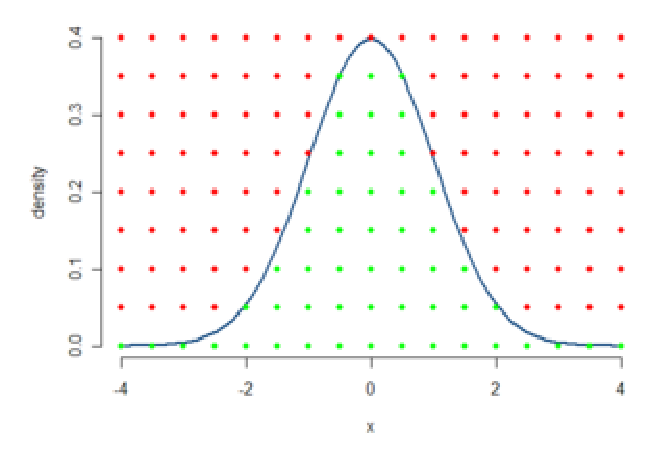
\includegraphics[width=\linewidth]{imgs/NormalRejectGrid.eps}
		\end{minipage}
		
	\end{frame}
	
	\begin{frame}
		\frametitle{Particular cases}
		
		Sometimes, we can benefit of mathematical transformations.\\
		The main weakness is that they are seldom compatible with variance
		reduction techniques.
		
		\mbox{}
		
		{\blue Example}: Box-Muller method for the normal law.
		
		\mbox{}
		
		{\red Idea}: it is easier to generate a point $(X, Y)$ from the bivariate
		normal law, of density on $\rit^2$
		\[
		f (x, y ) = \frac{1}{2\pi} e^{-(x^2 +y^2 )/2}.
		\]
		We change the cartesian coordinates $(X,Y)$ by the polar coordinates $(R, \Theta)$:\\
		\[
		R^2 = X^2 + Y^2 ; Y = R \sin \Theta.
		\]
		
		It gives an elegant approach, but incompatible with variance reduction techniques and slower than inversion.
		
	\end{frame}
	
\end{document}